\chapter{Approach}
\section{Description}
\Blindtext
\begin{figure}
\centering
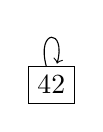
\begin{tikzpicture}
\node[draw] (one) {42};
\draw (one) edge [loop above] (one);
\end{tikzpicture}
\caption{A Figure with long long long long long long long long long long long
long long long long long long long long long long long text}
\label{fig:one}
\end{figure}


%% 
%% Mit Komascript können unterschiedliche Titel für Abschnittsüberschrift,
%% Seitenkopf und Inhaltsverzeichnis gesetzt werden 
%%
\section[tocentry={Text with table (TOC entry)},%
head={Text with table (page head)}]%
{Text with table (section heading)}
\Blindtext

\begin{table}
\centering
% Schöne Tabellen mit Booktabs
\begin{tabular}{rl}
\toprule
\textbf{a header} & \textbf{a header}\\
\midrule
something & important\\
something & important\\
\bottomrule
\end{tabular}
\caption{A Table}
\label{tab:one}
\end{table}

\section{Text with Formulae}
\blindmathpaper[8]
